%! Author = Len Washington III
%! Date = 2/15/24

% Preamble
\documentclass[lab={2},title={Voice Onset Time}]{com310lab}

% Packages


% Document
\begin{document}

\maketitle

\begin{overview}
	Consonants of all stripes can be classified as to whether they are voiced or voiceless, but the exact cut to voicing varies across consonant types as well as across different languages.
	For example, step consonants, regardless of voicing, generally show some degree of vocal fold vibration when they occur immediately before a vowel.
	Likewise, an acoustic cue that counts as voiced in one language many not count as voiced in another.\\

	A ``cue'' is a physical property of the speech that helps a listener correctly recognize a speech sound.
	For example, one cue to voicing for stop consonants is called ``voice onset time,'' or VOT, which refers to the time interval between when the articulators release after a closure and when voicing begins.
	Consider the VOT for a typical voiceless alveolar stop in American English, such as the \ipa{/t/} in `top':
	the tongue tip makes contact with alveolar ridge and makes a complete seal for a period of time.
	This period of closure is seen in a waveform as a period of silence and no detectable waves.
	Then, there is a release of the tongue tip, which can be seen as a sudden brief burst of acoustic energy (intense aperiodic waves).
	Following this, there is an interval of time when there is no voicing, but there is a period of low-frequency turbulence associated with aspiration.
	Lastly, voicing for the voicing for the vowel begins.
	This can be seen in a waveform when near-identical waves set up at regular intervals--around 1 wave every 10 milliseconds of so (1 second = 1000 milliseconds).\\

	VOT is measured from the moment of release to the moment voicing begins.
	It is reported in milliseconds.
	Figure~\ref{fig:vot} below shows different measurements of VOT\@.
	It can be a positive value when the release occurs before voicing begins (right waveform),
	it can be a negative value when voicing precedes the release (left waveform), and VOT is 0 when the release and voice occur simultaneously (middle waveform).

	\begin{figure}[H]
		\centering
		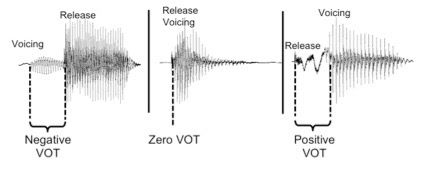
\includegraphics[width=\textwidth]{vot}
		\caption{Three different VOT values based on the onset of voicing relative to the release of active articulators.}
		\label{fig:vot}
	\end{figure}~
\end{overview}

\begin{problem}
	English makes a two-way distinction among stop consonants at each place of articulation: each is either voiced or voiceless.
	Thai makes a three-way distinction: stops are voiced, voiceless or voiceless aspirated.
	Hindi makes a four-way distinction among stops: they are voiced, voiceless, voiceless aspirated, or voiced aspirated.
	(Examples for the alveolar/dental and labial series for each language are given below.)
	However, it is unclear what physical property helps listeners distinguish among the different sounds.
	At issue is whether VOT is a reliable physical indicator of the different kinds of stop consonants and whether there is variation in VOT across the three languages.

	\begin{table}[H]
		\centering
		\label{tab:languages}
		\begin{tabular}{p{0.3\textwidth} *{5}{ p{0.08\textwidth} } p{0.15\textwidth}}
			& \multicolumn{2}{p{0.2\textwidth}}{\textbf{English}} & \multicolumn{2}{p{0.2\textwidth}}{\textbf{Thai}} & \multicolumn{2}{p{0.2\textwidth}}{\textbf{Hindi}}\\
			\textbf{Labial-series} & & & & & & \\
			voiced & \ipa{/ber/} & `bear' & \ipa{/ba/} & `crazy' & \ipa{/bal/} & `hair'\\
			voiceless aspirated & \ipa{/per/} & `pear' & \ipa{/p\super h{}a/} & `cloth' & \ipa{/p\super h{}a/} & `knife-blade'\\
			voiceless unaspirated & & & \ipa{/pa/} & `aunt' & \ipa{/pa/} & `take care of'\\
			voiced aspirated & & & & & \ipa{/b\super h{}al/} & `forehead'\\
			\textbf{Alveolar/dental-series} & & & & & & \\
			voiced & \ipa{/der/} & `dare' & \ipa{/da:/} & `curse' & \ipa{/dal/} & `lentil'\\
			voiceless aspirated & \ipa{/ter/} & `tear' & \ipa{/t\super h{}a:/} & `landing' & \ipa{/t\super h{}a/} & `plate'\\
			voiceless unaspirated & & & \ipa{/ta:/} & `eye' & \ipa{/tal/} & `beat'\\
			voiced aspirated & & & & & \ipa{/d\super h{}al/} & `knife'\\
		\end{tabular}
	\end{table}~
\end{problem}

\begin{task}
	Retrieve files containing stop consonants for English, Thai, and Hindi, using Praat and the guide above, measure VOT for all files.
	The files will be made available in a flash drive, and they will also be made available on a shared Google Drive file (check your email for an invitation to view the file folder).
	The file names correspond to the transcription and glosses (translations) above.
	A demonstration of how to measure VOT will be given at the beginning of the lab.\\

	Then, address the issue raised above: how does VOT distinguish among the various stop consonants with respect to voicing, and the extent you can, aspiration.
	Describe any variation in VOT across the three languages.
	Supply summary statistics and figures as needed.
	Report results for each language individually.
	Also, within each language, report results separately for the alveolar/dental stops and the labial stops.
\end{task}

\begin{writeup}
	Follow the format for writing up phonetics lab reports and upload your report on Blackboard.
\end{writeup}

\pagebreak

\labtitle

\begin{topic}
	Clearly state the topic that you are investigating.
	An example would be, ``This lab addresses the way adults talk to pets versus infants.''
\end{topic}

\begin{issue}
	A description of the issue at stake.
	An issue is the problem that you are attempting to solve.
	An example would be,
	``The special register of infant-directed speech is sometimes claimed to be intended to clearly contrary speech characteristics to language-learning infants, yet speech to prts would appear to share this same special register, and there is no suggestion that adults talk to pets in this way to help them learn language.
	At issue is whether pet- and infant-directed speech are, in fact, identical.''
	You only need to cite relevant information from our lectures, from the textbook, or from the lab instructions itself to motivate your issue, but however you decide to state the issue, be clear to draw out what is at state in addressing it.
\end{issue}

\begin{hypothesis}
	A statement of the research questions and hypotheses under investigation.
	A hypothesis is a tentative explanation for an (anticipated) observation of data.
	An example would be, ``Data were analyzed to address the issue of pet- vs. infant-directed speech.
	I predict that if speech directed to infants is intended to be clear, then such speech would have, among other properties, an expanded vowel space because xxx.
	In contrast, if pet-directed speech is diminutive and not intended for language-learning purposes, then such speech would be characterized as being merely loud speech and not show any expanded vowel space because yyy.''
	This particular hypothesis requires quite a bit of knowledge of phonetics, which you will not possess at the beginning of the semester.
	You should state a hypothesis as strongly as your knowledge of phonetics and speech characteristics allow.
	Don't go out on a limb and guess at things if you are uncertain.
\end{hypothesis}

\begin{method}
	A description of the method.
	An example would be,
	``In the lab activity, I recorded $x$ people saying $y$ words to $z$ pets, and then assume $x$ people saying the same words to $z$ infants.
	Then, I made the following measurements: $x$, $y$, and $z$.''
	Be specific.
	Explain what equipment you used, or how data were obtained.
	Define any measurements.
	An example would be,
	``Loud speech was defined as any speech with an average intensity of xxx, and expanded vowel space was defined as cases where [acoustic measures] showed yyy.''
\end{method}

\begin{results}
	A description of the results.
	An example would be,
	``Results indicated vowel space for pet-directed speech exhibited louder, longer segments, but not a bigger vowel space, consistent with the prediction that such speech is merely loud and not meant to help discriminate among speech sounds.
	In contrast, infant-directed speech \textit{did} exhibit an expanded vowel space, which I take as evidence as supporting the hypothesis that the special register to infants is for language learning purposes and is acoustically distinct from pet-directed speech.''
	Provide relevant tables, figures of (minimally) descriptive statistics where relevant.\\
\end{results}

\begin{discussion}
	A critical analysis of your study.
	An example would be,
	``While the study revealed a difference in pet- versus infant-directed speech, it does have some drawbacks.
	First, I didn't discuss whether infant-directed speech is actually effective in helping infants to discriminate among speech sounds.
	Moreover, vowel-space isn't necessarily a strong indicator of an attempt to teach an infant to discriminate among speech sounds in the first place.
	Rather, an equally plausible explanation could be that adults xxx.''
\end{discussion}

\end{document}